\documentclass[sigconf]{acmart}

\usepackage{booktabs} % For formal tables
\usepackage{algorithmicx}
\usepackage[ruled]{algorithm}
\usepackage{algpseudocode}


\definecolor{stringColor}{rgb}{0.8,0.1,0.1}
\usepackage{listings}
\lstdefinelanguage{JavaScript}{
  keywords={typeof, new, true, false, catch, function, return, null, catch, switch, var, if, in, while, do, else, case, break},
  morekeywords={reaction, preamble, language, actor, input, output},
  keywordstyle=\color{black}\bfseries,
  ndkeywords={class, export, boolean, throw, implements, import, this},
  ndkeywordstyle=\color{darkgray}\bfseries,
  identifierstyle=\color{black},
  sensitive=false,
  comment=[l]{//},
  morecomment=[s]{/*}{*/},
  commentstyle=\color{purple}\ttfamily,
  stringstyle=\color{stringColor}\ttfamily,
  morestring=[b]',
  morestring=[b]"
}
\lstset{
   language=JavaScript,
   backgroundcolor=\color{white},
   extendedchars=true,
   basicstyle=\footnotesize\ttfamily,
   showstringspaces=false,
   showspaces=false,
   numbers=left,
   numberstyle=\tiny,
   numbersep=5pt,
   tabsize=2,
   breaklines=true,
   showtabs=false,
   captionpos=b,
   xleftmargin=-5pt, xrightmargin=0pt
}

\newcounter{myctr}
\newenvironment{compactEnumerate}{\begin{list}{\arabic{myctr}.}
{\usecounter{myctr}
%\setlength{\topsep}{1mm}\setlength{\itemsep}{0.5mm}
\setlength{\topsep}{0.3mm}\setlength{\itemsep}{0mm}
\setlength{\parsep}{0.3mm}
\setlength{\itemindent}{0mm}\setlength{\partopsep}{0mm}
\setlength{\labelwidth}{15mm}
\setlength{\leftmargin}{4mm}}}{\end{list}}

% Copyright
%\setcopyright{none}
\setcopyright{acmcopyright}
%\setcopyright{acmlicensed}
%\setcopyright{rightsretained}
%\setcopyright{usgov}
%\setcopyright{usgovmixed}
%\setcopyright{cagov}
%\setcopyright{cagovmixed}


\copyrightyear{2019} 
\acmYear{2019} 
%\setcopyright{acmlicensed}
\acmConference[DAC '19]{The 56th ACM/ESDA/IEEE Design Automation Conference}{June 2--6, 2019}{Las Vegas, USA}
%\acmBooktitle{The 34th ACM/SIGAPP Symposium on Applied Computing (SAC '19), April 8--12, 2019, Limassol, Cyprus}
%\acmPrice{15.00}
%\acmDOI{10.1145/3297280.3297337}
%\acmISBN{978-1-4503-5933-7/19/04}



%\acmArticle{4}
%\acmPrice{15.00}

% These commands are optional
%\acmBooktitle{Transactions of the ACM Woodstock conference}
%\editor{Jennifer B. Sartor}
%\editor{Theo D'Hondt}
%\editor{Wolfgang De Meuter}

%%%%%%%%%%%%%%%%%%%%%%%%%%%%%%%%%%%%%%%%%%%%%%%%%%%%

\usepackage{amsmath}
\usepackage{amssymb}
\usepackage{subcaption}
\usepackage{multicol}
\usepackage[inline]{enumitem}
\usepackage{xcolor} 
\usepackage{ifthen}


%%%%%%%%%%%%%%%%%%%%%%%%%%%%%%%%%%%%%%%%%%%%%%%%%%%%
% Note style by Sebastian Ertel
%%%%%%%%%%%%%%%%%%%%%%%%%%%%%%%%%%%%%%%%%%%%%%%%%%%%

\newboolean{showcomments}
\setboolean{showcomments}{true} %set false for final submission
\ifthenelse{\boolean{showcomments}}
{ \newcommand{\mynote}[3]{
   \fbox{\bfseries\sffamily\scriptsize#1}
   {\small$\blacktriangleright$\textsf{\emph{\color{#3}{#2}}}$\blacktriangleleft$}}}
{ \newcommand{\mynote}[3]{}}
\definecolor{asparagus}{rgb}{0.53, 0.66, 0.42}

% One command per author:
\newcommand{\todo}[1]{\mynote{TODO}{#1}{red}}
\newcommand{\martin}[1]{\mynote{Martin}{#1}{blue}}% 
\newcommand{\marten}[1]{\mynote{Marten}{#1}{cyan}}% 
\newcommand{\isa}[1]{\mynote{Isabelle}{#1}{darkgreen}}% 
\newcommand{\ag}[1]{\mynote{Andr\'es}{#1}{asparagus}}% 
\newcommand{\armin}[1]{\mynote{Armin}{#1}{purple}}%

\begin{document}

\title{Actors, Time Stamps, and Determinism \\ for Time-Critical Systems}


\author{Marten Lohstroh}
\orcid{0000-0001-8833-4117}
\email{marten@eecs.berkeley.edu}
% \affiliation{%
% 	\institution{University of California, Berkeley}
% 	%\streetaddress{}
% 	%\postcode{}
% 	%\city{} 
% 	\country{USA} 
% }

\affiliation{%
	\institution{UC Berkeley, USA}
	%\streetaddress{}
	%\postcode{}
	%\city{} 
	% \country{USA} 
}

\author{Martin Schoeberl}
\orcid{1234-5678-9012}
\email{masca@dtu.dk}
\affiliation{%
	\institution{TU Denmark, Denmark}
	%\streetaddress{}
	%\postcode{2800}
	%\city{Lyngby} 
	% \country{Denmark} 
}

\author{Andr\'es Goens}
\orcid{}
\email{andres.goens@tu-dresden.de}
\affiliation{%
	\institution{TU Dresden, Germany}
	%\streetaddress{}
	%\postcode{}
	%\city{} 
	% \country{USA} 
}

\author{Armin Wasicek}
\orcid{}
\email{armin.wasicek@avast.com}
\affiliation{%
	\institution{Avast, USA}
	%\streetaddress{}
	%\postcode{}
	%\city{} 
	%\country{USA} 
}

\author{Christopher Gill}
\orcid{}
\email{cdgill@wustl.edu}

\affiliation{%
	\institution{Washington Univ., St. Louis, USA}
	%\streetaddress{}
	%\postcode{}
	%\city{} 
	%\country{USA} 
}

\author{Marjan Sirjani}
\orcid{}
\email{marjan.sirjani@mdh.se}

\affiliation{%
	\institution{M\"alardalen Univ., Sweden}
	%\streetaddress{}
	%\postcode{}
	%\city{} 
	%\country{Sweden} 
}

\author{Edward A. Lee}
\orcid{0000-0002-5663-0584}
\email{eal@eecs.berkeley.edu}

\affiliation{%
	\institution{UC Berkeley, USA}
	%\streetaddress{}
	%\postcode{}
	%\city{} 
	%\country{USA} 
}


\renewcommand{\shortauthors}{E. A. Lee et al.}

\begin{abstract}
Abstract
\end{abstract}

%
% The code below should be generated by the tool at
% http://dl.acm.org/ccs.cfm
% Please copy and paste the code instead of the example below. 
%
\begin{CCSXML}
	<ccs2012>
	<concept>
	<concept_id>10010520.10010553.10010562</concept_id>
	<concept_desc>Computer systems organization~Embedded systems</concept_desc>
	<concept_significance>500</concept_significance>
	</concept>
	</ccs2012>  
\end{CCSXML}

\ccsdesc[500]{Computer systems organization~Embedded systems}


\keywords{actor, real-time systems, worst-case execution time}

\maketitle 

\section{Introduction}\label{sec:intro}
Precision timing plays an important role in a plethora of modern systems, ranging anywhere from embedded control systems that continually interact with concurrent physical processes (i.e., cyber-physical systems) to large-scale distributed systems requiring some measure of consistency. In order to effectively program these systems, there is a need for programming models with a semantics that includes time. In current-day general-purpose hardware and programming languages, timing properties of software are emergent--not specified. Therefore, the verification of timing properties of time-critical systems often relies on rigorous testing, but effectively testing software in the face of non-determinism is extremely challenging. We propose an actor-oriented programming model that reduces non-determinism by introducing a semantic notion of time, allowing programmers to specify timing properties, which, if executed on capable hardware, can be guaranteed statically.

In this paper, we propose an actor-oriented programming model for time-critical systems, based on a discrete event semantics, which  
ensures that messages between actors are handled in deterministic order unless nondeterminism is introduced explicitly as a desired property. We introduce \emph{Lingua Franca} (LF), an interface definition language for the description of actors and their composition. LF allows programmers to implement the functionality of actors using a language of their choice. By default, all Lingua Franca programs will be deterministic. We use a semantic notion of time and time stamps to achieve this. 

% LF is designed with a pre-compilation step on polyglot principles, allowing an analysis step to make guarantees as well as opaque actors to serve as means to combine different systems. 

%This functionality will live inside actors, the interfaces of which will be described in Lingua Franca to be able to analyze global timing properties of the system. 
% Similarly desirable are guarantees, e.g. about meeting real-time deadlines, or sound properties, like determinism, which makes \emph{any} software easier to test and verify.
% However, the landscape of modern computing system is complex and very heterogeneous, which makes combining components already difficult, even more so enforcing a particular set of execution semantics. 

%is the transition here too rough?
\section{Actors}\label{sec:actor}
The actor model was introduced by Hewitt~\cite{Hewitt:77:Actors} in the early 70s. 
%A well-known programming paradigm used in this context are Hewitt~\cite{Hewitt:77:Actors} actors.
Since then,
%their introduction in the 70s,
the use of actors has proliferated in programming languages~\cite{Armstrong:96:Erlang,haller2009scala,desai2013p}, coordination languages~\cite{Arbab:04:Reo,ARC}, distributed systems~\cite{Hunt2018, DBLP:journals/corr/abs-1712-05889}, and simulation engines~\cite{Ptolemy:14:Book,DBLP:journals/fuin/SirjaniMSB04}. 
Actors have much in common with objects---a paradigm focused on reducing code replication by means of inheritance and increasing modularity via data encapsulation---but unlike objects, actors also provide a model for \emph{concurrency}. 
Indeed, each actor is presumed to operate concurrently alongside other actors that it may exchange messages with, asynchronously. 
These properties make actors an ideal for programming reactive systems. The lack of any guarantees with respect to the ordering of messages, and the absence of a notion of time, makes this a very general model, albeit a less useful one for the specification of systems in which timely execution and determinism are important.

Extra machinery can be introduced for the formal specification and analysis of systems composed of Hewitt actors.
For instance, Real-time Maude~\cite{olveczky:2008:real}, a timed rewriting logic framework and (temporal) model checking tool, has been applied to actors in~\cite{Ding2003}.
Similarly, the modeling language Rebeca performs analysis that uses a model checker to ensure that nondeterminism allowed in the model does not lead to behaviors that violate requirements of the simulated system~\cite{KHAMESPANAH2015184}.
Alternatively, constraints can be placed on actors' allowable behaviors so that they adhere to a well-defined model of computation (MoC), satisfying desirable properties such as deadlock freedom, schedulability, bounded memory usage, and deterministic execution, by construction. It is the latter approach we follow.

%\ag{I tried to sum-up the big picture to help with the structure. This is based on my current understanding. It's probably not up-to-date with your project I've understood so far, so please correct me where I'm wrong.}
%
%What is \emph{Lingua Franca}? 
%\begin{enumerate}
%  \item DSL (Dual to embedded: host language gets embedded into LF)
%    \begin{itemize}
%    \item Polyglot (Multi-language)
%    \item Concrete parser
%    \end{itemize}
%  \item A MoC (refining of actors)
%    \begin{itemize}
%    \item Formal specification
%    \item Concrete implementations (hosts)
%    \end{itemize}
%  \item An analysis Framework
%    \begin{itemize}
%    \item Annotations ``implicit'' from language
%    \item Concrete reasonings (e.g. WCET analysis?)
%    \end{itemize}
%\end{enumerate} 
%
%Advantages:
%\begin{enumerate}
%\item Multi-language and multi-system: allows combining (``glue'') and reuse of legacy systems and code.
%\item Concurrency and determinism.
%\item Encapsulation via scoping mechanisms.
%\item Analysis through interface definitions.
%\item A semantic notion of time.
%\end{enumerate}

%\section{Actors in Lingua Franca}
% sectioning.... ?
A key difference between Hewitt's notion of actors and actors in LF, is that rather than having actors address other actors directly, LF actors send messages via ports, completely agnostic of the presence or absence of downstream receivers. The connections between actors are embedded in a level of hierarchy---a composite---that is tasked with relaying messages between contained actors. While this approach increases modularity, more importantly, it exposes dependencies between actors that can be used to devise a schedule that ensures i) actors observe produced messages in time stamp order, and ii) actors cannot produce messages with time stamp $t$ until all anti-dependent inputs with time stamp $t$ are known. This is the same approach taken in the Discrete Event implementation of Ptolemy II~\cite{LeeEtAl:7:DiscreteEvents}, which is formally based on a synchronous reactive MoC~\todo{[Benveniste,Berry,1991]}, but, to increase efficiency, it averts performing a fixed-point computation by executing actors in topological order. That way, each actor is only executed once per tick of the logical clock. Because the schedule is determined based on the topology of the actor graph, no static analysis of the actors' internals is required---actors are treated as black boxes.

% also, no need for postfire % maybe mention that this optimization comes at the loss of the ability of handling some zero-delay feedback models...
\section{Lingua Franca}
In Lingua Franca, actors could be characterized as \emph{gray} boxes considering they reveal some key features of their internal structure, namely a closer approximation of the true dependencies between ports. Other than actors in Ptolemy II, which implement an abstract semantics~\cite{TripakisEtAl:12:AbstractSemantics} that requires each actor to perform all of its computation in a so-called \emph{fire} function, LF actors are broken down into smaller units we call \emph{reactions}. This approach, inspired by the characterization of dataflow processes given in \cite{LeeMatsikoudis:09:Dataflow}, exposes the dependencies between actors' inputs and output at a finer grain. We enforce simple lexical scoping rules, which virtually any programmer is already familiar with, to limit reactions' access to the actors' input and output ports, thereby eliminating dependencies between ports that are out of scope. The interface definitions of reactions are much like function definitions. Consider the following example which defines a brake component as an LF-actor:

\begin{minipage}{0.50\linewidth}
% \begin{enumerate}
%   \item First item \\
%         This is the second line in item and this may extend to third if long
%   \item second item\ldots
% \end{enumerate}
\begin{lstlisting}[numbers=none]
language ECMA6/Flow;
actor Brake {%
  input check:any
  input apply:number
  output on:boolean
  preamble 
\end{lstlisting}
\end{minipage}%
\begin{minipage}{0.50\linewidth}
\begin{lstlisting}[numbers=none]
  reaction(apply) -> 
  reaction(check) -> on 
%}
\end{lstlisting}
\end{minipage}%

\todo{Explain this, discuss polyglot}
\todo{Precisely because no static analysis is required...}

Having this finer-grained dependency information available at the interface level also opens up avenues for scheduling optimizations, makes the detection of zero-delay feedback less conservative, and, we conjecture, will enable remote procedure calls (RPCs) between actors without compromising determinism or modularity. The same dependency analysis performed to devise a schedule for message delivery and rule out zero-delay feedback can be used to coordinate RPCs and guarantee deadlock freedom. We think that integrating RPCs into LF will be key to achieving wide adoption of our programming model, because it is such a omnipresent language feature, even in highly popular (non-deterministic) actor-oriented frameworks such as Akka \armin{Not sure which part of Akka this refers to, but we've used Avro for RPC. (akka-remote would be somewhat more than plain RPC)}.

Central to the LF programming model is the relationship between the time stamps associated with the receipt of messages, which denote \emph{logical} time, and the passing of \emph{physical} time, approximated by the system time of the execution platform. While logical time can be sped up or slowed down arbitrarily in a simulation, the fact that actors can interact with the physical world through sensors and actuators requires that logical time and physical time ``keep up'' with one another in order to have a temporal semantics that obeys the principle of causality (i.e., effects cannot precede causes) for all observers. 

% Sort reactions topologically based on precedences.

% Global notion of “current time” t.

% Event queue containing future events.

% Choose earliest time stamp t’ on the queue.

% Wait for the real-time clock to match t’.

% Execute actors in topological sort order.

% \begin{figure}[ht]
% \begin{algorithmic}[1]
%  \Procedure{execute}{}
   
%  \EndProcedure
%  \end{algorithmic}
% \caption{The Lingua Franca execution engine \marten{Maybe too much detail}}
% \label{fig:lf-engine}
% \end{figure}

% Time is \emph{logical} time. This logical time be used for simulation and then
% we call it model time. We can also use the network of actors for the implementation
% of the system. 

% In that case wall clock time is used to timestamp input values
% at sensors. Logical time can never advance further than wall clock time.
% We have a notion of delay in two places: (1) as a delay actor to break up
% feedback loops (2) at actuators to specify that an actuation shall happen before
% (or exactly at) the logical time of the input plus the delay.

% Actors communicate via ports. All data exchanged has a timestamp.
% An actor does not advance time, the reaction is considered instantaneous.

% Reactions of one actor are atomic and are allowed to change state.
% Reactions are triggered by available inputs with timestamps at logical
% time (or older). When several reactions of an actor are enabled at the
% same time, the definition order in LF defines the execution order.

% A reaction of an actor can also be released by a trigger. A trigger
% can be periodic triggers or a single shot timer.
%The engine that drives the execution of LF actors (see Figure~\ref{fig:lf-engine}) enforces the following principles:
Before discussing a number of motivating examples, we summarize our model in terms of the following principles:

\begin{enumerate}
\item Messages exchanged between actors are timestamped;
\item The arrival of a message denotes a discrete event;
\item Actors carry input ports, triggers, output ports, state, and a list of reactions, each of which:
\begin{enumerate}
\item is triggered by the presence of an event on an input port (originating from another actor) or trigger (originating from the actor itself);
\item sees events in time stamp order;
\item can read/modify the actor's state;
\item can set the values of output ports it has access to;
\item can schedule \emph{future} events on triggers it has access to;
\item can read the values of input ports it has access to;
\begin{enumerate}
\item the time stamp associated with an observed event always denotes the current logical time; and
\item if no message arrives at a given port at the current logical time, its value is considered \emph{absent}.
\end{enumerate}
\end{enumerate}
\item No logical time elapses during a reaction;
\item Any two reactions of the same actor execute atomically with respect to one another; and
\item If two reactions of the same actor are triggered simultaneously, they execute in a predefined order;
\end{enumerate}

\martin{Some more things for the list: reactions that are ready have a release order
according to their definition order (in LF).}
\marten{See item (6)}
\martin{ We have discussed two different input ports:
those that are only valid during the logical time of the time stamp (what did we call them?)
and the ones that latch the value and are valid in future logical time as well.}
\marten{I think we called them input ports and triggers, respectively. See item (3)(a). If unclear, we should definitely improve the wording. Same for the terminology. We could also go for external/internal input ports. Internal ports are only referenced by the actor itself; both can be considered triggers...}

\section{Timing and Determinism}
\todo{discuss timing and scheduling using actor graph examples (no code)}
\subsection{Delays \& Deadlines}
$\mathcal{D}$
We have a notion of delay in two places: (1) as a delay actor to break up
feedback loops and (2) at actuators to specify that an actuation shall happen before
(or exactly at) the logical time of the input plus the delay.

Delays deserve also the purpose to align events with wall clock time and to
allow execution of reactions in their worst-case execution time (WCET).
The sum of all reaction's WCET from one synchronization point (either
sample of sensors or output of a delay actor) to another synchronization
point (or output of an actuator) has to be less than the delay.
\begin{figure}[ht]
 \centering
 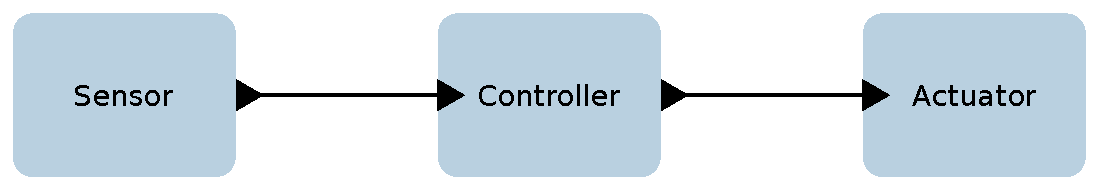
\includegraphics[width=\linewidth]{img/example-1}
 \caption{First example}
 \label{fig:example-1}
\end{figure}
% DAC Properties A1-9.
% Simple examples. Which should those be?
% First one to start with: sensor computation actuator
% Introduce notion of a deadline
% Why on the local platform, model should not get ahead.
% Example 1: Synchronization to real time and deadlines
% Example 2: Why delay has to wait
% Example 3: shut off the lights some time after the switch has been flipped.
% Reason to have the deadline definition as stated: detectability. Suppose the start deadline cannot be met; the
% reaction should not be carried out (and then the violation be reported on).
 
\subsection{Sporadic Events and Call Backs}

Sporadic events and call backs can trigger a reaction. This reaction is allowed
to observe and also change the state of the actor. Therefore, they are not allowed
to preempt a reaction (reactions are atomic to each other). To enforce this atomicity
a sporadic reaction is executed only between two logical timestamps $t_1$ and $t_2$.
This can be enforced on a C based host by turning off interrupts when executing
a reaction. Interrupts are enabled when all\footnote{\todo{All is a little bit restrictive,
just for state atomicity we would not need to wait for all reaction, just for a single.
But there is another issue that this shall happen only between two timestamps.
I don't recall the details.}}
reactions for timestamp $t_1$ have been executed and disabled again when logical
time is advanced to $t_2$ where all reactions for $t_2$ are executed.

\subsection{Causality}
We do not want to run ahead of realtime, because actors can produce spontaneous events that need to be stamped with 
pysical time, and we don't want these timestamps to be ``in the past.''

\begin{figure}[ht]
 \centering
 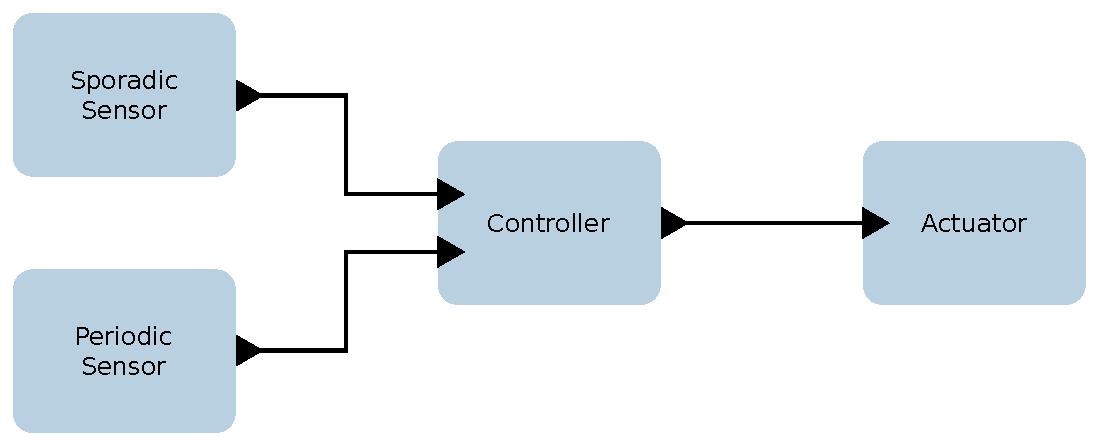
\includegraphics[width=\linewidth]{img/example-2}
 \caption{Second example}
 \label{fig:example-2}
\end{figure}


\subsection{Example 3}
Shut off the lights some time after the switch has been flipped. Reason to have the deadline definition as stated: detectability. Suppose the start deadline cannot be met; the reaction should not be carried out (and the violation be reported on subsequently).

\begin{figure}[ht]
 \centering
 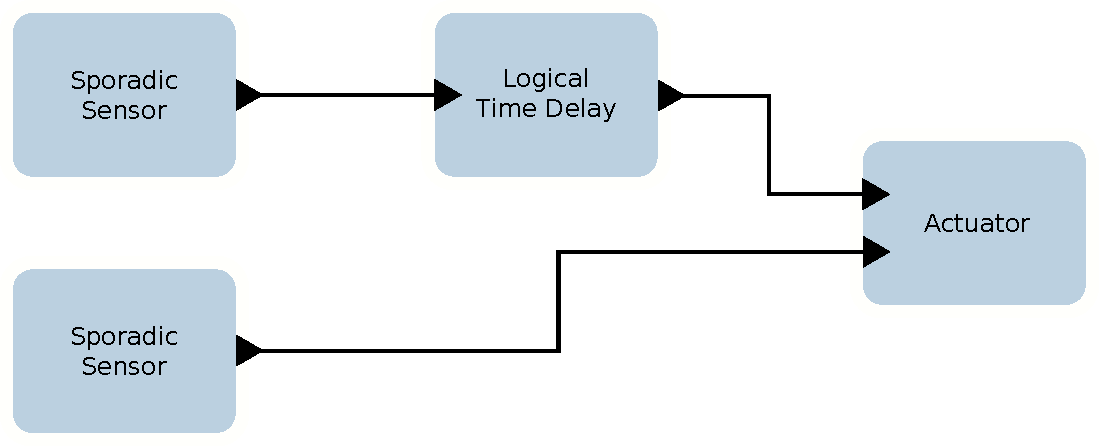
\includegraphics[width=\linewidth]{img/example-3}
 \caption{Third example}
 \label{fig:example-3}
\end{figure}

\marten{In third example, discuss how persistent ports can be used.}
\marten{Also, discuss optimized scheduler that runs ahead of physical time.}
\section{Related Work}
\label{sec:related}

Towards a real-time coordination model for mobile computing \cite{hackmann2005towards}
Method and tools for mixed-criticality real-time applications within PharOS \cite{lemerre2011method}
Accessors \cite{brooks2018component}
S-Net~\cite{grelck2008gentle}
Guarded Atomic Actions~\cite{Rosenband:2004:MSG:996566.996583}
Timed C \cite{Broman_timedC}
%\section{Actors}
%


% Constraints can be placed on actors' allowable behaviors so that actors adhere to a well-defined model of computation, satisfying desirable properties such as deadlock freedom, schedulability, bounded memory usage, and deterministic execution by construction. This has been the guiding principle in the Ptolemy project\footnote{\url{https://ptolemy.berkeley.edu/}}, which studies modeling, simulation, and design of concurrent, real-time, embedded systems.

% Several frameworks have been built based, loosely or strictly, on the
% original Hewitt actor model
% \cite{Hewitt:77:Actors,Agha:97:ActorComputation}, including Akka
% \cite{AkkaAction2016},
% Ray \cite{DBLP:journals/corr/abs-1712-05889}, and Rebeca
% \cite{DBLP:journals/fuin/SirjaniMSB04}. One property of the original
% Hewitt actor model is that messages received by an actor from distinct
% sources are handled in nondeterministic order. \marten{even messages from the same source can arrive out-of-order}


% \martin{We need to check this: Outputs generated by a time triggered
% reaction are timestamped. When the system is simulated, the timestamp
% is equal to the model time. When the system is used for execution, the logical
% time for the release of the reaction is synchronized to wall clock time and therefore
% the output message are synchronized to wall clock time.}



% \martin{We have (and maybe support) two options: (1) input is only valid when
% the timestamp equals logical time, absent at other times or (2) keeping the value
% of an input for future logical time and having a default value for system initialization time.
% (in the JS accessors this is the way it is specified, the default value gives the
% ``keep'' or persistent semantic).}

\section{The Lingua Franca Compiler Tool Chain}
% Time is \emph{logical} time. This logical time be used for simulation and then
% we call it model time. We can also use the network of actors for the implementation
% of the system. In that case wall clock time is used to timestamp input values
% at sensors. Logical time can never advance further than wall clock time. \marten{Not entirely true: an optimized scheduler can do this under very specific circumstances that we'll elaborate on in the example.}


% The scheduler invokes reactions of actors dependent in inputs with timestamps
% that are equal (or earlier--can this happen?) at logical time $t_1$.
% Logical time cannot advance further than wall clock time $t_w$. If next logical
% time $t_2 > t_w$ the scheduler waits till $t_w \ge t_2$.




\todo{Describe that the single threaded execution of JavaScript enforces
the restriction of the call back not interrupting the reaction.}




For dynamic systems, e.g., an IoT that keeps running, but in different contexts
(e.g., places), we support dynamic reconfiguration of the network of actors.
This may be well supported when targeting a dynamic language such as JavaScript,
but harder to implement in C.

To support reconfiguration we need a more complete language than the configuration
language LF. Therefore, our first iteration of dynamic reconfiguration is done in the
host language JavaScript. In that case, the host language needs access to actors and
ports. However, we can use scopes to having access to those parts of the framework
only in well defined places.


\section{Conclusions}
\label{sec:conclusion}


\subsection*{Acknowledgments}
The work in this paper was supported in part by the National Science Foundation (NSF),
award \#CNS-1836601 (Reconciling Safety with the Internet) and the iCyPhy Research Center
(Industrial Cyber-Physical Systems, supported by Avast, Camozzi Industries, Denso, Ford, Siemens, and Toyota
%The work presented in this paper was partially funded by the
%Danish Council for Independent Research \textbar{} Technology and Production Sciences
%under the project PREDICT\footnote{\url{http://predict.compute.dtu.dk/}}
%contract no.~4184-00127A.

% Please do not add any references to msbib.bib.
% They get lost when I 'generate' it again.
\bibliographystyle{ACM-Reference-Format}
\bibliography{Refs} 

\end{document}
